%\documentclass[12pt]{article}
%\usepackage{amsmath}
%\usepackage{graphicx, color}
%\usepackage{amssymb}
%\usepackage{listings} %source code listing
%\usepackage{multirow}
%%\usepackage[version=2]{mhchem}
%\usepackage{subfig}
%\usepackage{hyperref}
%\usepackage{units}
%\usepackage{gensymb}
%\usepackage{adjustbox}
%\usepackage{listings}
%\usepackage{color}
%\usepackage{tcolorbox}
%\usepackage{tabularx}
%\definecolor{codegreen}{rgb}{0,0.6,0}
%\definecolor{codegray}{rgb}{0.5,0.5,0.5}
%\definecolor{codepurple}{rgb}{0.58,0,0.82}
%\definecolor{backcolour}{rgb}{0.95,0.95,0.92}
%
%\newcommand{\specialcell}[2][c]{%
%  \begin{tabular}[#1]{@{}c@{}}#2\end{tabular}}
% 
%
%
%\title{Reactor physics with Python \\ Lecture Notes}
%
%
%\author{Zs.~Elter. E. Branger, M. Preston \\ Uppsala University \\
%        Division of Applied Nuclear Physics}%\corref{cja}}
%%
%\date{2021.}
%\begin{document}

\section{Introduction}

Nuclear reactors play an important role in our modern society. In some countries, such as France  the major part of electricity is produced from nuclear power. Over the last decades, we have gathered a great deal of knowledge and experience in designing nuclear reactors, but we must remember that nuclear reactors are very complex, therefore it is important to sustain this knowledge, and train professionals with the necessary understanding to operate or build new reactors. This lecture note is intended for students and professional with a basic understanding of nuclear power generation, but with no prior or little knowledge of nuclear reactor physics, who either want to gain a basic understanding of the principles of nuclear reactor theory or are motivated to follow more advanced studies in the future.

The complexity of nuclear reactors arises from the fact that there are several phenomena happening in a nuclear reactor at different scales, which interplay: heat production from nuclear fission, heat transfer and fluid dynamics. In some context reactor physics can refer to all of these phenomena, however traditionally reactor physics is meant to be limited to describing the physics within the reactor core, where the nuclear fuel and the coolant can be found and intends to describe the transport of neutrons within the core. This text is also limited to studying the reactor core, and it intends to provide an introductory, often phenomenological description to convey the main concepts, and to serve as a good basis for future advanced studies. Figure \ref{fig:reactorcore} stand here to highlight that indeed from the whole system of a nuclear power plant, our interest is during the text only the neutron physics happening inside the reactor vessel: within the nuclear fuel, the coolant material and the control elements. 

The aim of this lecture note and the related datalab exercises is to teach through (hopefully) pedagogical examples which can be implemented as small programs. It is however important to highlight that this text is a \textit{lecture note}, it does not intend to cover everything and include every important derivation, only the ones said during the lectures. The note had two intentions: to provide scientific figures created with python, so the students can have access to the source code of the figures and to give a summary of the lectures in order to aid the lecturer during teaching. However a student reading this text will need to review further literature to grasp the subject. The following books can provide great help:

\begin{itemize}
\item Duderstadt, James J.: Nuclear reactor analysis (referred to as D\&H during the note)
\item Lewis, E. E.: Fundamentals of nuclear reactor physics
\item Lamarsh, John R.: Introduction to Nuclear Reactor theory
\item Bell, George and Glasstone, Samuel: Nuclear Reactor Theory (referred to as B\&G during the note)
\item W. Stacey: Nuclear reactor physics
\item C. Demaziere: Physics of nuclear reactors (lecture notes)
\item Z. Szatmary: Introduction to reactor physics (although only for Hungarian speakers)
\end{itemize}

In fact during the writing of these notes we have heavily relied on these books. Mostly we have tried to follow D\& H, but we have used other books, where they provided a more illustrative explanation or derivation. Some parts of these lecture notes will therefore show some similarities to these books. We will however not include a reference for every single equation in the notes, nevertheless at some point we will point out the right book for further reading.

\subsection{Nuclear reactors}

As we said earlier the reader of these notes is expected to have a basic familiarity of nuclear plants and reactors. If that is not the case, please read for example D\& H Chapter 3-II, here we just provide a brief introduction to introduce the terminology used in this text.

\begin{figure}[ht!]
\protect \centering{
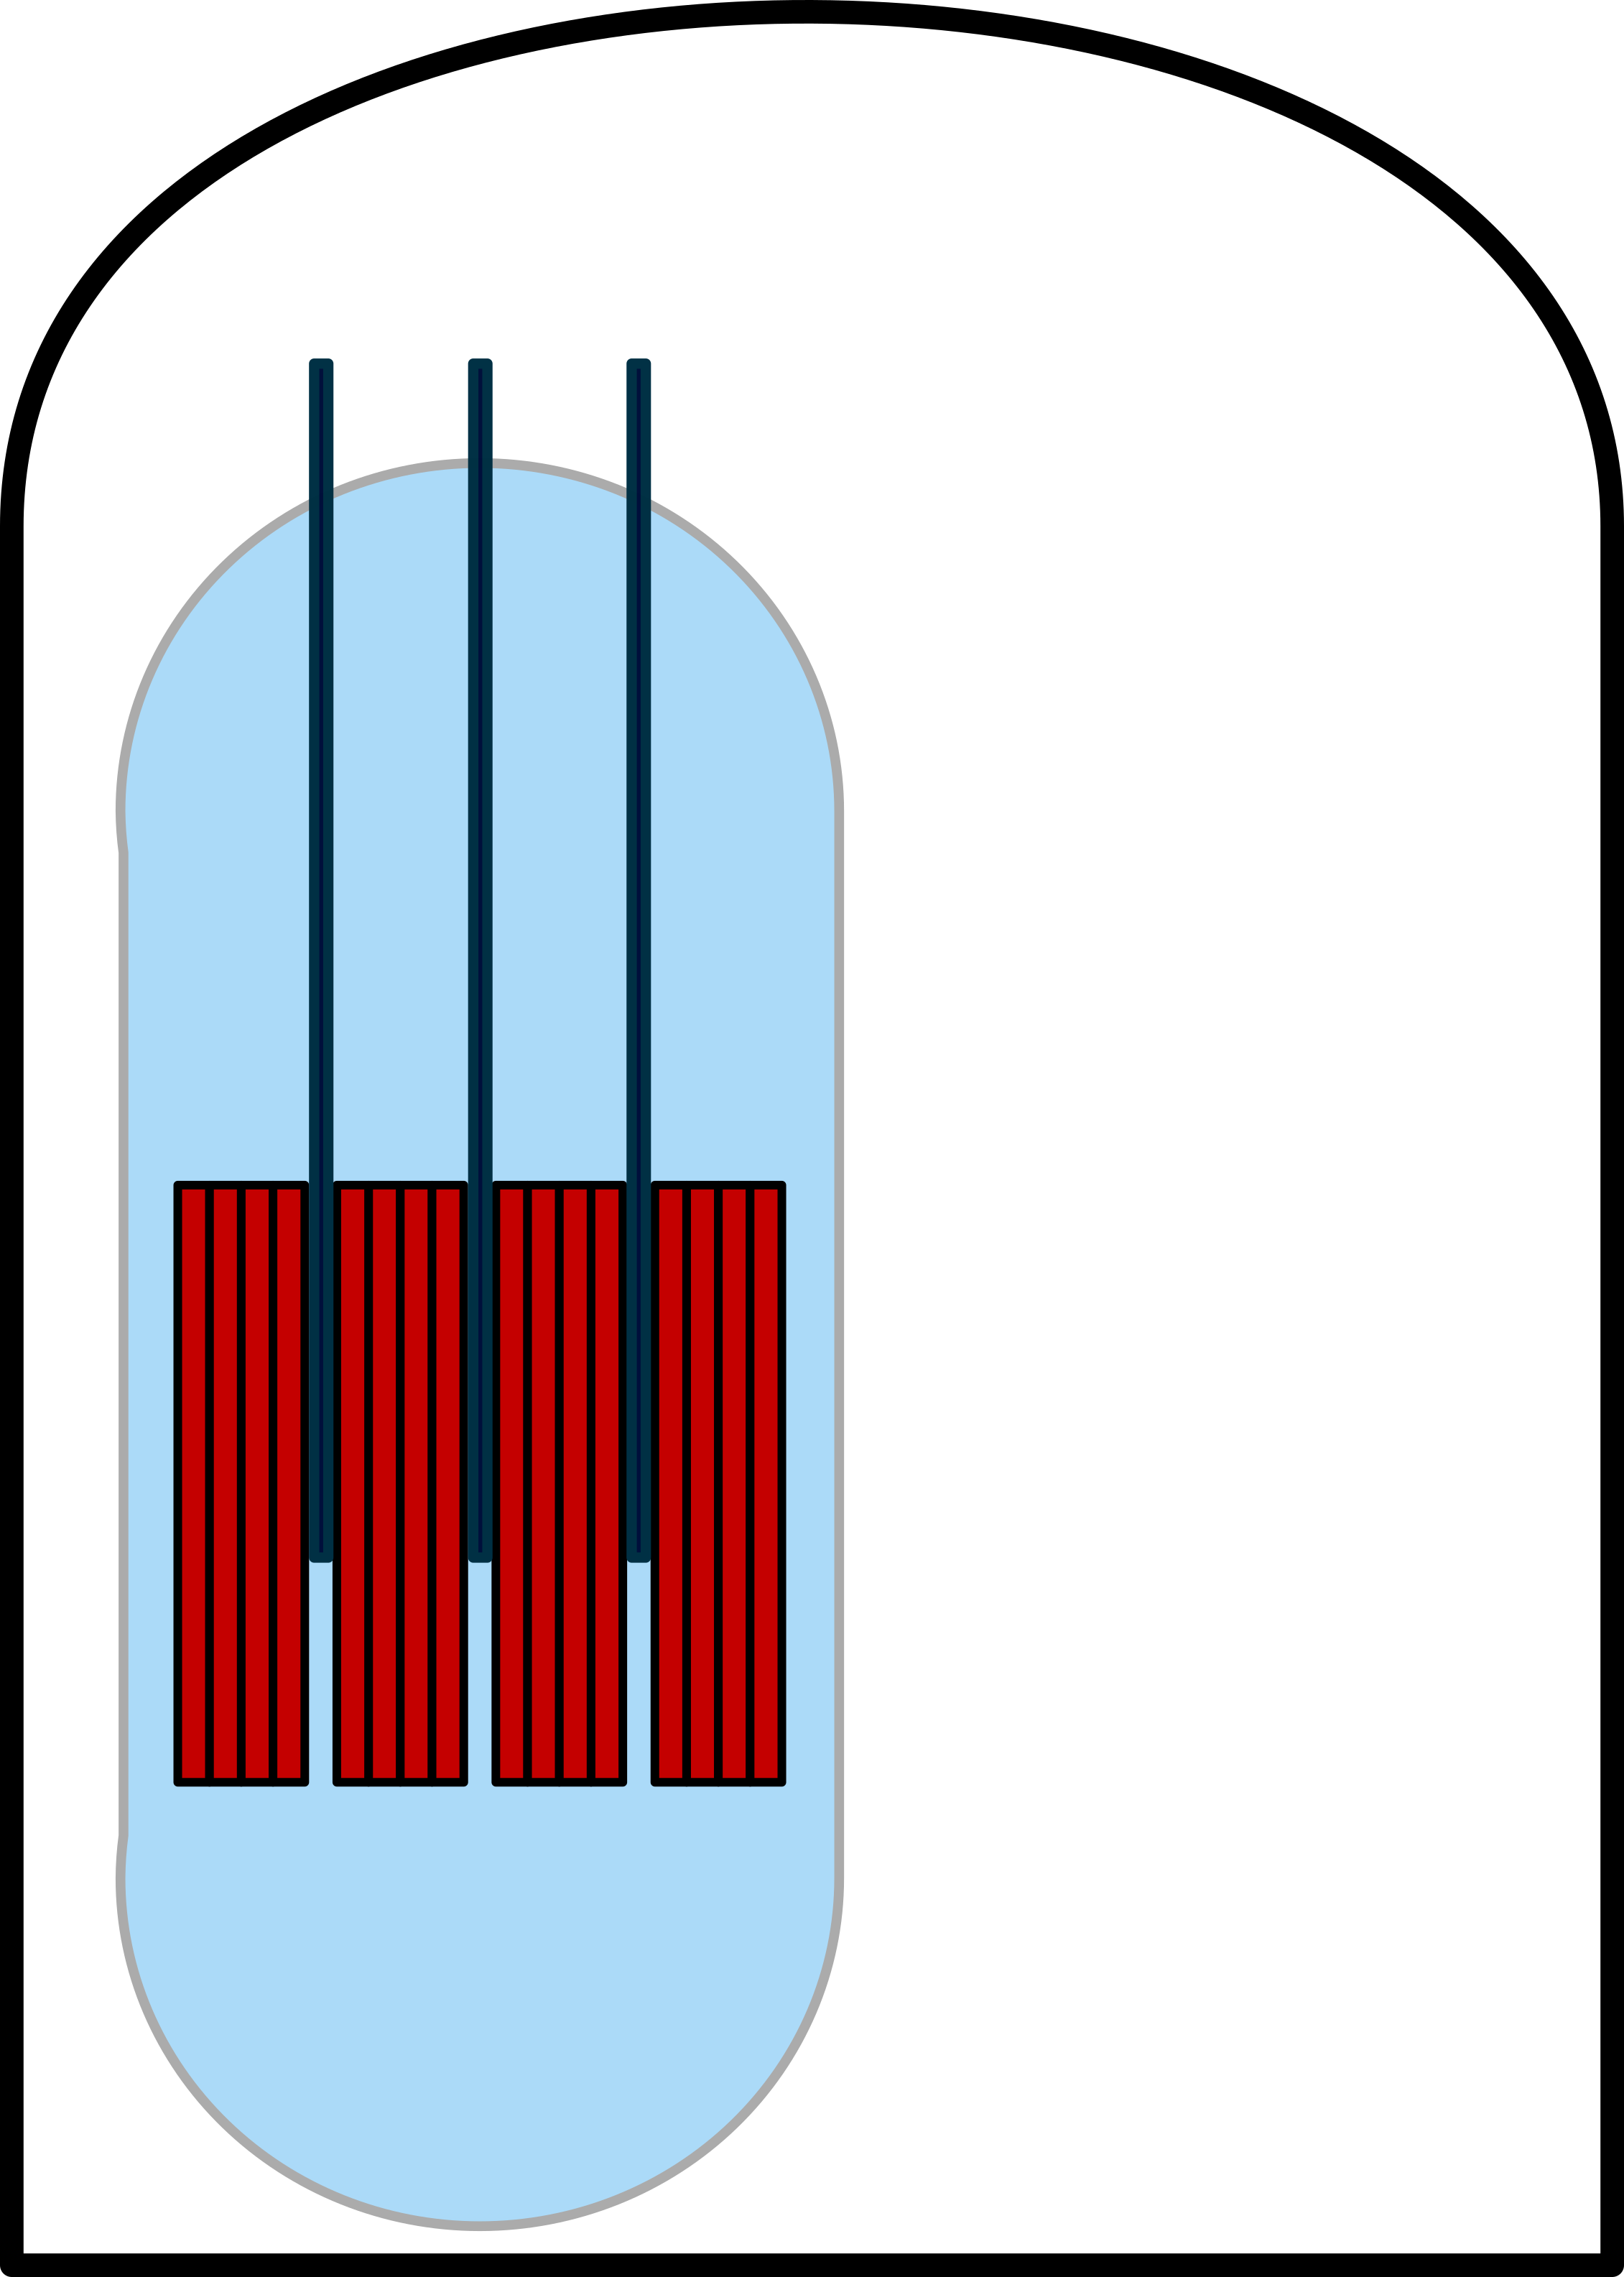
\includegraphics[scale=0.36] {figures/00-reactorofinterest.png}}\protect
\caption{\label{fig:reactorcore} \footnotesize{The part of the power plant which is of interest for the subject of this lecture note: the reactor core.}}
\end{figure}

As said earlier the focus of this text is on the heart of the nuclear power plant: the reactor core. Also, the main focus of this text is going to be Light Water Reactors (LWR), since to this reactor type is the most widespread. The reactor core of an LWR is located in a pressure vessel and is built of nuclear fuel, coolant channels, structural and control elements. Typically we also require some sort of monitoring of the core, therefore usually various instrumentation systems are placed in the core. The fuel is made of uranium in the ceramic form of uranium-dioxide (often referred to as UOX, or UO$_2$). As we will see later, the uranium might be enriched: the weight fraction of the fissile isotope uranium-235 is higher than in natural uranium. The UOX material is formed into small cylindrical \textit{pellet}s, which are placed in a metallic, often zirconium tube, the \textit{cladding}. The tube is filled usually with an inert gas, and sealed. This tube is called a \textit{fuel pin} or \textit{fuel rod}. The fuel pins are then placed in a \textit{bundle} or \textit{assembly}. Western type fuel assemblies are usually rectangular lattices, whereas eastern type assemblies have a hexagonal lattice. Figure \ref{fig:assembly} shows the layout of a 17x17 pressurized water reactor (PWR) assembly, which contains 25 control rod positions in \textit{guide tubes}. The fuel assemblies are arranged into a lattice (again depending on the type of the reactor this might be rectangular or hexagonal) which makes up the core, with a close to cylindrical shape. In some reactors the core is surrounded by non-fuel assemblies (\textit{reflectors} and \textit{shielding}), or fuel elements which have special use (for example \textit{breeding blankets}). Later we will discuss these in more detail. Table \ref{table:pwrsize} summarizes the typical sizes of a PWR reactor. 

\begin{figure}[ht!]
\protect \centering{
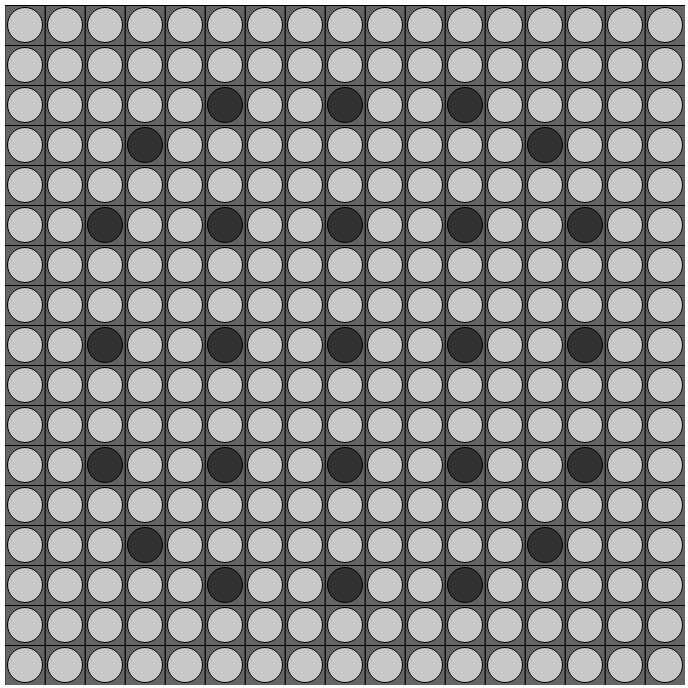
\includegraphics[scale=0.26] {figures/00-assembly.png}}\protect
\caption{\label{fig:assembly} \footnotesize{A 17x17 PWR assembly lattice (darker positions highlight the control rods).}}
\end{figure}

\begin{table}\caption{Typical size of a PWR core}\label{table:pwrsize}
\begin{tabular}{c c}
Core diameter & 3-4 meters \\
Core height & 4 meters \\
Assembly width & 20 cm \\
Pin diameter & 1.0 cm \\
Pin pitch & 1.2 cm
\end{tabular}
\end{table}


\subsection{Reactor physics}

As mentioned before, the main subject of this text is reactor physics. However, even this can be split into further parts:

\begin{itemize}
\item Neutronics: to determine the distribution of neutrons in time, in energy, and in space for a given geometry and material configuration.
\item Depletion or burnup studies: Investigate how the material composition changes in the reactor core over time: how much fissile material is lost, how much transuranic elements and fission products are created. 
\item Experimental reactor physics: Provide measurement methods which can be used to determine various quantities important during reactor operation.
\end{itemize}

In this text we will mainly focus on neutronics, and touch upon depletion. We will first introduce the relevant part of nuclear physics in order to describe reactions which might happen with neutrons traveling in a reactor. Then we will discuss how a neutron looses its kinetic energy in a nuclear reactor (this is the subject of \textit{slowing down}), and in fact at the end of its life it reaches thermal energies (this is the subject of \textit{thermalization}). Then we will derive a \textit{neutron transport} equation describing the balance between the production and loss of neutrons in the reactor. Then we will investigate how the number of neutrons changes in the reactor over time if we increase the probability of neutron survival (for example by removing control rods). And finally we will leave behind the subject of neutronics, and study how the nuclear fuel evolves due to long-term irradiation and how this affects the neutron transport.

It must however mentioned, that the book is also a good introduction to neutron physics in general, that is a large portion of the text (on basic nuclear physics, neutron slowing down and neutron transport, neutron activation) is applicable even in non-multiplying media, which has practical relevance outside of the nuclear industry.  

\subsection{History of reactor physics}

Introducing the history of a subject before the subject has always the risk that parts are not going to be clear. Nevertheless, we have decided to outline first the history of reactor physics first, because it is both exciting pedagogic to see how great minds came up with ideas which at the end let to the widespread use of nuclear reactors.

\begin{tabularx}{\textwidth}{c | X}
1895 & Wilhelm R\"ontgen discovers X-rays  while testing various types of vacuum tubes. \\
1896 & Henri  Becquerel noticed that uranium ore emits similar radiation. \\
1898 & Marie and Pierre Curie shows that in fact three types of radiation is emitted. They discover radioactivity. \\
1911 & Rutherford discovers the nucleus while investigating the scattering of alpha-rays. But the discovery makes it difficult to explain the mass of the nucleus. \\
1932 & James Chadwick discovers the neutron. He uses the reaction $\text{He-4} + \text{Be-9} \rightarrow \text{C-12} + \text{n}$. Such reaction needs energetic alpha particles. With his discovery finally the nucleus mass and beta-decay can be explained.
 
Even more important it was discovered that the neutral particle can penetrate the nucleus therefore it became possible to convert it.  The study of nuclear reactions, modern alchemy has began (mostly with a PoBe source, where the alpha-decaying Polonium is mixed with Beryllium). \\
1934 & Frederic Joliot-Curie and Irene Curie noticed after the absorption of a neutron, a beta-decay might follow (induced radioactivity), and the element is transmuted into an other element. 
\end{tabularx}

\begin{tabularx}{\textwidth}{c | X}
1930s & Enrico Fermi's team systematically tried to transmutation reactions for several isotopes. They found that upon performing the neutron activation experiments under water, the induced radioactivity is much higher. Fermi thus started to develop the theory of neutron slowing down and found that, the initially fast neutrons scatter on the hydrogen atoms, and they reach thermal energy (when the speed is comparable to that of thermal motion). They also found that by activating uranium they can produce elements heavier than the ones existing in nature: neptunium and plutonium. \\
1938 & Fermi receives the Nobel for this work. \\
1938 & When Otto Hahn and Fritz Strassmann repeated the activation experiments of uranium they observed several beta decays, which couldn't be explained by the transuranic element. From the reaction products they managed to separate Barium. Then Lisa Meitner realized that uranium had to undergo fission, and infact it is the fission products which emit the unaccounted beta-radiation. \\
1933 & (Note that we jumped back in time!) Leo Szilard comes up with the idea of a chain reaction: if the product of neutron activation produces new neutrons these neutrons could be used for further reactions. He patented the idea of a nuclear reactor, already before he even knew about fission. He assumed that there has to be a reaction which results in a neutron which can self-sustain the reaction. And with the discovery of fission this became obvious. Also that we can produce a lot of energy in this way. 
\end{tabularx}

\begin{tabularx}{\textwidth}{c | X}
1939 & Leo Szilard becomes conscious about the possibility of building a nuclear bomb and convinces Albert Einstein to write a letter to President Roosevelt about the potential of a nuclear bomb, and the threat of Germany already developing it (after all they discovered fission). They stopped all publications on the subject. The Manhattan Project started, during which they realized that there are two ways of making such a bomb: with uranium-235 or plutonium-239. The first option needed separation from U-238 (since in nature the weight fraction of uranium-235 is low), which proved to be difficult at that time (the separation couldn't be based on chemistry, had to be based on the slight difference in mass). The second option required the neutron activation of uranium-238. To carry out such reactions at scale, a large amount of neutrons were needed, which couldn't be produced with the typical neutron sources of the time. This required a chain reactor. \\
1942 & Chicago-pile. By placing UO2 rods (made of natural uranium) in hole of graphite bricks the first controlled chain reaction was achieved. It gave a proof of concept for chain reaction and also allowed the discovery of that there are enough delayed neutrons, thus the chain reaction can be controlled. \\
1944 & The Hanford reactor was built for plutonium production. Chemical reprocessing methods were used to separate plutonium from uranium. \\
1945 & Was a sad year of reactor physics. \\
1951 & EBR-1 fast reactor was built and produced electricity. \\
1955 & Obninsk Nuclear Power Plant, first nuclear station was built and produced a whooping 6MW power.
\end{tabularx}

And then the era of nuclear power stations started, building hundreds of reactors both for energy production and for research.


\subsection{Programming with python}

Of course as the name of the course shows "with Python" is appended to reactor physics. Reactor physics in practice requires a lot of computations from numerical solutions of differential equations through handling large amount of nuclear data till processing measured results. Our experience is that the best way to learn reactor physics is by applying it in practice, therefore it was decided that the lectures will be complemented with 11 datalabs, where students can develop simple simulations of neutron transport, perform data analysis, and also use more advanced Monte Carlo codes. It was decided that students will use Python and its mainstream libraries for these tasks. The main reason is that Python has a very simple syntax, thus students can quickly learn it. Also, it was important that the simulations we will develop are intended to help the understanding of reactor physics, thus it would not have been ideal if the complexities of some programming language hindered us. We acknowledge that for advanced reactor physics, where computational efficiency and time is crucial, Python might not be the preferred choice.

Nevertheless, in this lecture note it is not going to be apparent that this course is a "python" course. The only place where Python occurs in the notes is behind the scenes: the scientific figures were created with Matplotlib, the plotting library of Python, with the aim that the source code can be distributed along the figures, to be transparent and to help understanding the data behind the figures. 

We strongly hope that students performing all the datalabs while reading the lectures will become proficient users of Python. Nevertheless, we have to emphasize that the main goal of having programming exercises during the datalabs is to help students understand the basic theory of nuclear reactors and neutron transport.

%\end{document}